\chapter{Muon Generation}

Muons can originate through cosmic rays or neutrinos considering the natural production processes and neglecting acceleration experiments e.g. the LHC.
While most of the muons going downward in the detector, originate from cosmic rays, after $\mathcal{O}(\num{1e4})$ meter-water-equivalent (mwe) event the highest energetic muons lost all their energy and stopps.
Therefore muons seen as upward-going events in a detector originate from neutrino interactions, as neutrinos can propagate through the entire earth without any interaction.

\section{Cosmic Ray induced Muons}

\subsection{Cosmic Ray Energy Spectrum}

Cosmic Rays hit the atmosphere with a rate of \SI{999}{\milli\hertz} and consist of mainly Protons and Helium nucleus, as can be seen in the energy spectrum in figure \ref{}.
Until energies of roughly a GeV cosmic rays from outside of our solar system are screened by the Heliosphere.
Therefore the main source in this region is the sun resulting in a rather flat energy spectrum.

Above a GeV the magnetic fields of sun are not powerful enough to accelerate particles to such high energies and galactic sources play the main role.
Until energies of a PeV, a region called \enquote{knee}, the main sources are considered supernova remnants.
Supernovae occure once in a century in our galaxy, while their shock waves propagate hundreds of years into the interstellar medium.
The particles with these energies are considered to undergo the so called Fermi acceleration, a shock acceleration resulting in a power law spectrum $E^{-\gamma}$ with an index of $\gamma = \num{2}$.
Due to interaction losses and (TODO: entweichen) the spectrum gets steeper and results in a measured spectral index of \num{2.7}.

Between the \enquote{knee} and the so called \enquote{ankle} at an EeV yet unknown processes, probably Pulsars or Quasars, become dominant and increase the spectral index to \num{3.1}.
Above the \enquote{ankle} sources inside our galaxy are not powerful enough and extragalactic sources, e.g. Active Galactic Nuclei, become the main contributor.
The resulting spectral shape flattens again to an index of \num{2.6}.
At around \SI{1e20}{eV} the protons interact with the photons of the cosmic microwave Background (CMB) to a Delta resonance, resulting in the GZK-cutoff of the energy spectrum.
The CMB is a left-over from the big bang when the temperature drops below the critical value to perform electromagnetic pair production and annihilation.
Due to the expanding universe, the temperature of the CMB is today at \SI{2}{K}.

% \begin{figure}
%     \centering
%     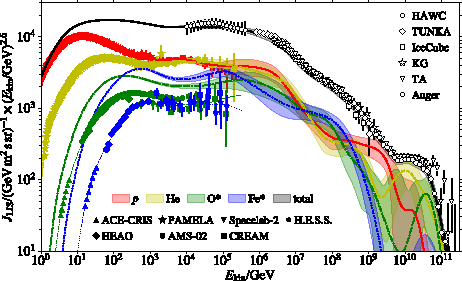
\includegraphics[scale=1]{./images/cosmic_ray_spectrum.pdf}
%     \caption{The energy spectrum of the Cosmic Rays for all Compositions from the GeV range to the GZK-cutoff.}
%     \label{fig:cr_spectrum}
% \end{figure}

\subsection{Cosmic Ray induced Air Showers}

When cosmic rays reach the earth they interact with the dense medium of the atmosphere.
Depending on the energy and the composition the height of the first interaction is at \SIrange{10}{15}{km}.
The secondary particles of this interaction again interact with the atmosphere resulting in a particle cascade or Air shower of thousands or even millions of particles.
These showers can be categorized into a hadronic, muonic and electromagnetic subshowers, that are illustrated in figure \ref{}.

% \begin{figure}
%     \centering
%     \includegraphics[scale=1]{./images/air_shower_illustration.pdf}
%     \caption{Scetch of an cosmic ray induced air shower illustrating the different subshower components.}
%     \label{fig:air_shower_components}
% \end{figure}

\textbf{The electromagnetic showercomponent} mainly consist of electrons, positrons and photons.
Starting e.g. with a high energy photon the two main processes are the production of an electron-positron pair and Compton Scattering.
While the latter is just important for the deflection, the pair production is the important process for the shower development.
The produced electron or positron dominantly loose their energy via Bremsstrahlung, creating again a high energy photon.
The Positron can also annihilate with the atomic electrons creating a photon pair.

(TODO: vgl Tau-Regeneration; wie viel Energie geht in einem cyclus verloren?)
The cylce of photon pair production and electron/positron bremsstrahlung contnues until the bremsstrahlung photons are not below an MeV and therefore not energetic enough to create an electron/positron pair.
Due to the high number of charged particles (\num{999} at \SI{999}{GeV}) that are created, this shower component produces the dominant amount of Cherenkov light and is also important for the radio signal of a shower.
The production of a muon pair is a subdominant process as the muon mass 200 times higher than the electron mass decreasing the phase space and is therefore not important for the em shower development.
Otherwise it is a non-negliable process regarding the number of produced muons, while the main production poriginates from the hadronic shower.

\textbf{The hadronic showercomponent} mainly consist of the lightest mesons, Pions \SI{999}{MeV} and Kaons \SI{999}{MeV}.
Due to their relatively long livetimes of $\tau_\pi = \SI{999}{\micro\second}$ and $\tau_K = \SI{999}{\micro\second}$ they propagate and loose some amount of energy through interactions, before they decay.
Pions decay mainly into muons, as their rest mass is just slightly higher.
Kaons either directly decay into muons or first decay into Pions, which then decay to muons and neutrinos.
The energy losses during the propagation of the Pions and Kaons lead to a steepening of the resulting muon and neutrino energy energy spectrum with a spectral index of \num{3.7}.
Muons or neutrinos originating from these processe are called \enquote{conventional atmospheric} Muons or Neutrinos.

Next to Pions and Kaons also short-lived Mesons and baryons occure in hadronic showers.
They consist mainly of mesons with a charm quark, like the D-Meson or the $\Lambda$-Baryon.
Due to their short livetime, they are not losing energy during a propagation and directly decay.
The resulting energy spectrum of the decay products therefore remains the same as the primary spectrum and the spectral index does not change.
Although these processes is subdominant, the smaller spectral index makes it relevant at higher energies.
Because of the direct decay of the hadrons, which mainly consist of charmed mesons, the resulting muons or neutrinos are called \enquote{charmed} or \enquote{prompt atmospheric} muons or neutrinos.

\textbf{The muonic showercomponent} mainly originates from the hadronic showercomponent and produce just a few secondaries compared to the other shower particles.
The high muon mass compared to the electron also decreases the interaction probability as the bremsstrahlung cross section goes with $1/m^2$.
Combined with the relatively high lifetime the muon range through dense media is the highest, neglecting neutrinos, making them the biggest background for all particle detectors even deep underground.
Except of detectors at high altitude, like HAWC or LHASSO, they are the only shower component measured on the earths surface, neglecting the em-radiation part like Cherenkov light, Fluorescence light or the radio signal.

The resulting muon and neutrino energy flux from cosmic ray induced air showers is shown in figure \ref{}.

% \begin{figure}
%     \centering
%     \includegraphics[scale=1]{./images/atmo_muo_neutrino_flux.pdf}
%     \caption{Atmospheric muon and neutrino flux using MCEq.}
%     \label{fig:atmo_mu_nu_flux}
% \end{figure}

A lateral shower profile and the contribution of the different subshower types is shown in figure \ref{}.
An increasing number of particles during the beginning of cascade developement can be seen as well as a decreasing part when more and more Bremsstrahlung photons are too low energetic for elelctron pair production.
The resulting maximum of the lateral shower profile $X_{\mathrm{max}}$ at roghly \SI{5}{km} varys for the different primary particle types and energies making it an important feature for primary particle tagging.

% \begin{figure}
%     \centering
%     \includegraphics[scale=1]{./images/air_shower_lateral_profile.pdf}
%     \caption{Lateral shower profile of a \SI{999}{TeV} proton as primary particle.}
%     \label{fig:air_shower_profile}
% \end{figure}

\section{Muons from Neutrinos}

\subsection{Neutrino Energy Spectrum}

The neutrino energy spectrum shown in figure \ref{} is assumed to starts with a high number of cosmological neutrinos or the cosmic neutrino background (C$\nu$B).
Like the CMB they are left-overs from the big bang when the temperature drops below the critical value of weak lepton production and annihilation.
It consist of all neutrino flavours but the energies are far too low to be measured.

From the keV until the MeV region solar neutrinos from fusion processes dominate the spectrum.
At MeVs terrestial anti-neutrinos from natural radioactive nuclids or nuclear reactors contribute to the spectrum depending on the location on earth.
Although only electron neutrinos are produced in radioactive decays or fusion processes, solar neutrinos are measured in all three flavours through neutrino oscillation.
As the distance between the earth and the sun is greater than the oscillation length, which is not the case for terrestrial distances.
Furthermore in the MeV range neutrinos from supernova remnants also contribute to the spectrum.
For the last seen supernova SN1987A, where the neutrino contribution was first measured, the neutrino flux was orders of magnitudes higher than the SNR flux, dominating the spectrum at MeVs during the burst.
Here the distances are large enough for neutrino oscillation and a neutrino expectation of all three flavours.

For neutrino energies starting at GeVs cosmic ray induced atmospheric neutrinos are the main contributors.
Their contribution can be described by a broken power-law flux of \enquote{conventional} and \enquote{prompt} atmospheric neutrinos as described in section \ref{}.
Assuming pure pion decay, the resulting flavour ratio $\nu_e : \nu_mu : \nu_\tau$ is $1:2:0$.
\begin{align}
    \pi^+ \to &\mu^+ \nu_\mu \\
    &\mu^+ \to e^+ \nu_e \bar{\nu}_{\mu}
\end{align}
However, as the muons interact and loose nearly all of their energy before they decay, the so called \enquote{muon damping} model results in a $0:1:0$ flavour ratio, as the others are not measurable for neutrino telescopes.

At around \SI{100}{TeV} both the prompt and the astrophysical component are supposed to start dominating the flux.
While the astrophysical flux has already been measured by IceCube, the prompt component has always been fitted to zero and its contribution remain hidden, yet.
A distinct astrophysical neutrino source has also not been measured yet.
An often discussed candidate for astrophysical sources are Active Galactic Nuclei (AGNs).
The neutrino creation process for AGNs or other cosmic accelerators is similar to the atmosheric neutrinos, that accelerated protons interact with material near the source and the pion and muon secondaries produce neutrinos.
In contrast to the atmospheric neutrinos the medium at the source is not as dense as the atmosphere, so the pions and muons don't lose much of their energy before they decay.
Therefore the energy spectrum does not get steeper and the spectral index remains on the level of the fermi acceleration near 2.
In Addition the oscillation length is small compared to the distance changing the flavor ration at earth to $1:1:1$ assuming the pure pion decay model.
For the muon damping model, assming a more dense source region, the flavor ration after oscillation results in $9:9:9$.

At \SI{10}{PeV} neutrinos from the Delta-resonances at the GZK-cutoff, called cosmogenic neutrinos are predicted.
Unfortunately they have not been measured yet, as the detectors to measure them with radio techniques are currently in the planing fund raising phase.

Independent of the neutrino creation model at the astrophysical source, neutrinos of all three flavours will arrive at the earth through neutrino oscillation, including tau neutrinos.
While tau neutrinos are of special interest due to their high confidence in beeing of astrophysical origin, the created tau lepton also decays into muons making them a non-negligable source of neutrino induced muons.

\subsection{Neutrino Interactions}

There are three different interaction modes, illustrated in figure \ref{}, on how neutrinos can interact with matter.
% \begin{figure}
%     \begin{subfigure}{0.3\textwidth}
%         \centering
%         %
\begin{tikzpicture}
\begin{feynman}
    % define vertices
    % muon
    \vertex (nu_in) at (-\feynlen, \feynlen);
    \vertex (nu_vertex) at (0, 0.75*\feynlen);
    \vertex[right=2*\feynlen of nu_in] (l_out);
    % nucleus
    \vertex[below=1.5*\feynlen of nu_in] (n_in);
    \vertex[below=\feynlen of nu_vertex] (n_vertex);
    \vertex[below=1.5*\feynlen of l_out] (n_out);
    % draw diagram
    \diagram* {
        (nu_in) -- [fermion] (nu_vertex) -- [fermion] (l_out),
        (nu_vertex) -- [boson, edge label=$W^\mp$] (n_vertex)
    };
    % draw extra features with tikz (not available in tikz-feynman)
    \draw[thick, double] (n_in) -- (n_vertex) -- (n_out);
    \draw[fill] (nu_vertex) circle[radius=\feynvertexsize];
    \draw[fill] (n_vertex) circle[radius=\feynvertexsize];
    % add labels
    \node[left] at (nu_in) {$\nu_{l^\pm}$};
    \node[right] at (l_out) {$l^\pm$};
    \node[left] at (n_in) {$N$};
    \node[right] at (n_out) {$X$};
\end{feynman}
\end{tikzpicture}
%
%         \caption{Charged Current (CC)}
%         \label{fig:feyn_nu_cc}
%     \end{subfigure}
%     \hfill
%     \begin{subfigure}{0.3\textwidth}
%         \centering
%         %
\begin{tikzpicture}
\begin{feynman}
    % define vertices
    % muon
    \vertex (nu_in) at (-\feynlen, \feynlen);
    \vertex (nu_vertex) at (0, \feynlen-\feynsmallen);
    \vertex (nu_out) at (\feynlen, \feynlen);
    % nucleus
    \vertex (n_in) at (-\feynlen, -\feynlen);
    \vertex (n_vertex) at (0, -\feynlen+\feynsmallen);
    \vertex (n_out) at (\feynlen, -\feynlen);
    % draw diagram
    \diagram* {
        (nu_in) -- [fermion] (nu_vertex) -- [fermion] (nu_out),
        (nu_vertex) -- [boson] (n_vertex)
    };
    % draw extra features with tikz (not available in tikz-feynman)
    \draw[thick, double] (n_in) -- (n_vertex) -- (n_out);
    \draw[fill] (nu_vertex) circle[radius=\feynvertexsize];
    \draw[fill] (n_vertex) circle[radius=\feynvertexsize];
    % add labels
    \node[left] at (nu_in) {$\nu$};
    \node[right] at (l_out) {$\nu'$};
    \node[right] at (0,0) {$Z^0$};
    \node[left] at (n_in) {$N$};
    \node[right] at (n_out) {$X$};
\end{feynman}
\end{tikzpicture}
%
%         \caption{Neutral Current (NC)}
%         \label{fig:feyn_nu_nc}
%     \end{subfigure}
%     \hfill
%     \begin{subfigure}{0.3\textwidth}
%         \centering
%         %
\begin{tikzpicture}
\begin{feynman}
    % define vertices
    \vertex (nu_in) at (-\feynlen, 0.75*\feynlen);
    \vertex (e_in) at (-\feynlen, -0.75*\feynlen);
    \vertex (nu_vertex) at (0, 0);
    \vertex[right=\feynlen of nu_vertex] (w_out);
    % draw diagram
    \diagram* {
        (e_in) -- [fermion] (nu_vertex) -- [fermion] (nu_in),
        (nu_vertex) -- [boson] (w_out)
    };
    % draw extra features with tikz (not available in tikz-feynman)
    \draw[fill] (nu_vertex) circle[radius=\feynvertexsize];
    % add labels
    \node[left] at (nu_in) {$\bar{\nu}_e$};
    \node[left] at (e_in) {$e^-$};
    \node[right] at (w_out) {$W^-$};
\end{feynman}
\end{tikzpicture}
%
%         \caption{Glashow Resonance}
%         \label{fig:feyn_glashow}
%     \end{subfigure}
%     \caption{The feynman diagrams of the most dominant neutrino interactions at high energies.}
%     \label{fig:feyn_nu}
% \end{figure}

The Charged Current (CC) interaction, with a W-Boson as exchange partner between the nucleon and the neutrino
While the neutrino converts into its charged counterpart lepton the other outgoing product is the hadronic cascade.
The Neutral Current (NC) Interaction, with an Z-Boson as exchange partner just produces an energy loss of the neutrino without converting it.
Therefore just a hadronic cascade comes out of this interaction as a visible part.
Both for the CC and NC interactions in average a third of the neutrino energy is stored as hadronic cascade and two thirds in the outgoing lepton.
The CC interaction is the dominant interaction contributing two thirds to the total cros section, while the NC just contribute a third, as shown in figure \ref{}.
For lower energies the anti neutrino cross section is smaller as the valence quarks are the main interaction partners.
The sea quarks and thereby an equal treatment of neutrino and anti-neutrino become more important at higher energies.

At an energy of \SI{6.3}{PeV} the Glashow resonance dominates the cross section.
At this energy the anti-electron neutrino interactes resonantly with an atomic electron producing a W-Boson.
The result is a huge hadronic cascade, as the W-Boson decays with the hole energy producing also multiple higher energetic muon tracks characteristic for the this interaction.
The IceCube detector has seen one very likeli Glashow-resonance event after 10 years of data taking.

% \begin{figure}
%     \centering
%     \includegraphics[scale=1]{./images/air_shower_lateral_profile.pdf}
%     \caption{Lateral shower profile of a \SI{999}{TeV} proton as primary particle.}
%     \label{fig:air_shower_profile}
% \end{figure}
The total cross section for all interaction types is shown in figure \ref{} and for the CC and NC interaction the differential cross section is shown in figure {}.

(TODO: An energy distribution of the muons coming out of a glashow resonance or a hadronic cascade or em shower)

\chapter{Muon Detection}

Muons can be measured by the energy losses along their propagated track, each producing a particle cascade.
These secondaries can be detected by their emitted Cherenkov light, Fluorescence light or the produced radio signal.
Here the two main detection techniques of muons for cosmic ray detectors and for neutrino telescopes are presented.

\section{Detection principales}

The main detection mechanisms to detect Cosmic ray and neutrino induced showers are the Cherencok and the Askaryan effect.

\textbf{The Cherencov Effect} comes into role when charged particles are propagating faster than the speed of ligh in that medium.
The polarised medium during the propagation creates a signal.
When the charged particle propagates faster than the light, these signals are emitted coherently creating a Cherenkov cone (see figure \ref{}).
An analogon to this is the Airforce jet creating a hypersonic cone.
Around \num{1e5} Cherenkov photons are emitted per centi meter resulting in an energy loss of \SI{999}{MeV.\per.m} which is 5 orders of magnitude below the Ionization loss.
The wave length dependency of the emitted Cherenkov Photons are described in the Frank-Tamm-Formula and therefore mainly seen as ble light due to the quick absorption of higher energetic photons.


\textbf{The Askaryan Effect} is a combination of several radio signals.
The gemagnetic effect seperates the positrons and electrons creating a horizontal Dipole.
In addition to that there are just atomic electrons not poritrons cresating a vertical Dipole as the shower front pushes these electrons in front of it.
The combination of this horizontal and vertical Dipole creates a radio pulse.
When the energy of the shower gets high enough, this radio pulse can be detected.
The energy loss due to this effect is neglidgable.
The wavelength are in the order of meters and is therefore not absobed as quickly as CHerenkov Photons.

\section{Air shower Detectors}

There are multiple approaches to measure the different signals an air shower produces, from the direct particle detection at high altitudes over the muon detection at the surface to the Fluorescence or radio signal besides a shower.

Extended Airshower Arrays are placed at high altutudes, ideally near the typical $X_{\mathrm{max}}$ to measure most of the produced particles inside the detector.
Currently the most performand one operating is the HAWC detector at an altitide of \SI{4.2}{km} in Mexico.
On an area of \SI{22000}{\square\meter} 300 tanks each containing \SI{188}{\cubic\meter} of water and 4 PMTs measure the Cherenkov light emitted by the throug-going particles of the shower.
Although HAWC was mainly designed to measure Gamma Ray induced air showers, one can also use it to analyse cosmic ray showers in the PeV range.

The Pierre Auger Observatory operates at lower altitudes (\SI{999}{m}) with 1500 water cherencov tanks on an area of \SI{300}{\square\kilo\meter} each containg \SI{999}{\cubic\meter} water.
It was designed to detect the highest cosmic rays and teh energy spectrum at the GZK cut-off.
In addition to the surface detectors it also contains 24 Fluorescence telescopes measuring the lateral shower profile.
While the Water Cherencov tanks have a duty cycle of nearly \SI{100}{\percent} the Fluorecence detectors can only operate at clear nights limiting their duty cycle to \SI{20}{\percent} isch.
The emitted Fluorescence light at each shower depth is equivalent to the energy loss per distance making the energy of the shower extractable via the integral of the shower profile.
In combination with the shower profile on the ground measured by the surface detectors the main information of the primary particle, composition, energy and direction are reconstructed.

In principle, the number of detected muons on the ground would also be a good proxy.
Unfortunately there is a descrepancy ofthe measured data beeing \SI{60}{\percent} higher than the Monte Carlo simulation.
This is also known as \enquote{Muon Puzzle}.
The systematic uncertainties in the muon propagation and the electromagnetic models can in maximum just explain \SI{5}{\percent} of the missmatch.
It is considered, that most of the discrepancy arises from the uncertainties of the hadronic interaction models.
While most of the models are influenced by accelerator measurements like the LHC, these models provide good agreements for high transversal moments.
In the forward direction, the beam pipe and not a detector is located, which is good for those experments as most differential cross sections diverges in the forward direction.
Unfortunately the astroparticle physics most often measure the shower in the forward direction leading to less cross checks with the accelerator measurements.
This type of challange to evaluate cross section also in the forward direction does not just occure for the hadronic models, but for all types of particle interaction including the muon cross sections.

\section{Neutrino Detectors}

Most neutrino detectors use the  Cherencov light emitted by charged secondary particles to measure neutrinos.
Large volumes of media transparent to the blue Cherenkov light like Water, Ice or simply the air is used as a detection volume..
Other methods like the radio detection are in the developement phase.

\subsection{IceCube}

The biggest neutrino telescope is the IceCube detector located at the geographic southpole.
On a hexagonal grid of a square kilometer 78 Strings are drilled into the glacial ice with a string distance of \SI{125}{m}.
Each string contains \num{60} Digital Optical Modules (DOMs) equally placed between a depth of \SI{1500}{m} and \SI{2500}{m}.
Each DOM contains a Photomultiplier looking downward and measauring the emitted Cherenkov light.
The surrounded detection volume contains a cubic kilometer of ice measuring neutrinos energies between from \SI{100}{GeV} to \SI{10}{PeV}.
For higher energies the event rate is too small and in addition IceCube would be completely filled out with Cherencov light.

In the middle of IceCube 8 Strings each with 60 DOMs of higher quantum efficiency are placed more closely together.
This extension called \enquote{DeepCore} decreases the lower threshould for neutrino energies to \SI{10}{GeV} and uses the rest of IceCube as veto region.
Another extension is \enquote{IceTop} where a water cherencov tank is placed at the surface of each string.
This can either be used as an air shower detector at an altitude of \SI{3}{km} with the benefit of IceCube as a further muon detector to deeper analyse the atmospheric muons.
On the other side it works as a veto for IceCube to destinguish filter down-going neutrinos from atmospheric muon events as the neutrinos should not be seen in IceTop.

There is currently a proposal (or white paper?) for an extension of IceCube named IceCube-Gen2.
An extension called \enquote{IceCube-Upgrade}has already been funded to test new types of DOMs for Gen2.
Gen2 will enlarge the detected volume to \SI{8}{\cubic\kilo\meter} and will be place around IceCube.
(Im Gegensatz) to IceCube, the Strings in Gen2 will be orgenized on a sunflower structure avoiding corridors how muons can sneak inside and fake a cascade-like signal.
In addition to that a radio detection is planned, placing the antennas on grid with an inner distance of a kilometer and covering an area of \SI{100}{\cubic\kilo\meter}.

\subsection{Event Signatures}

The measured event signatures are devided into tracks and cascades.
NC neutrino interactions of all flavour have just a visible hadronic shower, which is as rather spherical cascade.
The additional electron of a CC interaction of electron neutrinos just propagate around 10 meters in the ice.
As this distance is pointlike for IceCube, the resulting cascade also has a spherical structure.
Although there are differences in the shower developments of em and hadronic cascades, especially through the later decays of neutral hadrons, it was not possible to distinguish between electromagnet and hadronic cascades \cite{MainzAnalyse}.

The greater mass of muons compared to electrons make them lose their energy much slower and travel multiple kilometers  through ice.
From the hadonic cascade of a muon neutrino CC-interaction vertex a long track is going out.
Therefore muon neutrinos do not have to interact inside the detection volume and can also interact far before the detector with the muons traveling inside, increasing the effective detector volume.

Tau leptons have an even higher mass than the muons and therefore a smaller energy loss resulting in a thin propagation track.
But the small lifetime of \SI{999}{ns} make the decay directly or for higher energies let the travel \SI{50}{m} per PeV.
The event signature depends on the decay channel; two-thirds are hadronic cascades and the last third is equally distributed between the muonic and the electronic channel.
Until energies of around \SI{100}{TeV} the second hadronic or em-cascade can not be destinguished from the first hadronic cascade at the neutrino vertex.
For higher energies these two cascades gets seperated more clearly and a double cascade or double bang signature is created.
The muonic tau decay also contributes to the amount of incoming muons starting before the detector.
For events starting inside the detector the outgoing track is smaller compared to the hadronic cascade as the additional neutrinos from the tau decay take away some enrgy.
For higher energies the thin tau track goes over to a brighter muon track.
But these differences in the track signature can just be seperated statistically for a number of events and not on an event level due to the stochasticity of the propagation.
Due to the limited resolution there has been just one promising tau neutrino event seen with IceCube after 10 years of measurement.

\subsection{Event selection}

The main interesting features to be reconstructed are the primary particle type, its energy and the direction.
To get the primary particle type a \textbf{classification} has to be made between the different event signatures; cascades and tracks.

A pure cascade sample contains mostly NC events and atmospheric electron neutrinos with CC interactions and less tau neutrinos.
Cascade searches uses the outer DOM layers as veto region against through-going muons, which detection rate is orders of magnitudes higher.
But even in DeepCore muon tracks are contaminating when traveling in teh middle between the Strings.
Also the stochasticity of the propagation processes, allowing muons to travel without visible losses and then deposit all of their energy in a catastrohic loss inside the detector.
As these processes are rare, an accurate description of the muon physics even at the tails or edges of the total and differential cross section is needed.

The tracks are further seprarted between upgoing and downgoing tracks.
Down-going events are mostoften atmospheric muons reaching the detector as bundels with a lateral distance of some meter between them.
Those events are seen one bright track as the limited resolution (verhindern) a seperation the single muons of a bundle.
An approach to analyse atmospheric muons using the bundels is the search for a leading muon containing most of the bundel energy.
A bundle of many low energetic events creates a bright track with a continuous energy loss.
Leading or single muons have a high stochasticity, e.g. with a huge bremsstrahlung loss resulting in a thiner track with brighter cascades on it.

Another approach to use atmospheric muons are stopping muons.
They mostoften single muons and have energies of just several GeV when enetering the detector.
At these energies they are in the regime of the minimal Ionization and can be used to measure the DomEfficiency.
Or using the direction and range, one can unfold the energies of the muons at the surface of the ice.

Up-going tracks can just be neutrino induced muons as muons can propagate large distances through the earth.
Unfortunately a simple extraction these muons with a zenith cut is not satisfying as the resulting sample is still dominated by misreconstructed muons.
Although the directional resolution is high for tracks, sometimes it can exceed \SI{5}{\degree} and contaminate the sample.
Therefore advanced machine learning algorithms are used to extract a purified sample.
The filtered track events are an ideal single muons sample at all energies; good to analyse the muon physics, e.g. the energy loss profile.
Just for the starting events, the hadronic cascade of the neutrino interaction contaminates a little bit.

\subsection{Event Reconstruction}

The directional resolution for tracks is compareably high (\SI{0.5}{\degree}) while being low for cascade events (\SI{5}{\degree}).
When the cascade is contained the energy resolution is high due to the calorimetric measurement.
For tracks, just a portion of the muon energy loss is deposited inside the detector and the energy is reconstructed using the energy loss per distance $\mathrm{d}E/\mathrm{d}X$, which goes nearly linear with the muon energy (c.f. section \ref{}).
For starting tracks, the energy resolution for the muons and neutrinos increases, due to the additional information of the hadronic cascade at the vertex.
For low energy muons the average energy loss is not proportional to the muon energy.
As these muons are mostoften stopping inside the detector, the track length can be used to reconstruct the energy.

For the energy reconstruction of the muons, the track inside the detector is splitted into multiple segments and the high energetic, stochastic losses are cutted away to get the continuous energy loss.
Furthermore these segments can be used to retrieve an energy loss profile by unfolding the energy losses per segment.

The ice properties with its different absorption and scattering lengths at different layers as well as the anisotropy are one of the largest systematic uncertainties for analysis at the IceCube detector.
Another systematic uncertainty is the DOM efficiency, varying the amount of light that is detected by $\pm\SI{5}{\percent}$.

\section{Further High Energy Neutrino Detectors}

Further neutrino telescopes using the detection principle like IceCube are the ANTARES/Km3Net experiment in the Mediterean sea, the Baikal/GVD in lake Baikal and the P-ONE experiment in the Bassin bay in front of Vancover.
Compared to IceCube these telescopes are upgrading to a cubic kilometer volume and are placed in water.
A comparison of the different scattering and absorption lengths are listed in table \ref{}.
`
To detect even higher energetic neutrinos and analyse the predicted cosmogenic neutrinos, detectors to measure the radio signal are under developement.
Because of the long wave length, these radio pulses can propagate a kilometer through the ice.
There are currently two attempts to build an Radio-Neutrino Detector; one as part of IeCube-Gen2 in the Antarctic Ice and another one on Greenland.

Another often use attempt to measure neutrinos is looking for events coming from earth and search for hadronic showers as just neutrinos can propagate through the earth.
The ANITA experiment consist of radio antennas on a ballon.
During the flights around the Antarctic cricle, it measures the radio signals coming from the earth.
Pierre Auger is looking for showers going upward are extreamly inclined showers.
If they measure not just the muon component but also the electromagnetic shower inside their surface detectors, the shower must have started deep inside the atmosphere only neutrinos can create.
HAWC looks at showers coming from the mountain next to it and MAGIC looks at the Atlantic if view to the stars is not clear but the view to the sea.
Both again looking for a hadronic shower, only Tau Neutrinos can produce.
For all these exeriments again atmospheric muons are the dominant background by orders of magnitudes.
Therefore an accurate description for all energies and energy losses is crucial to cover also the edge cases in the simulations.

\chapter{Muons Cross Sections}
\label{sec:cross_section}

The muon cross sections described in this chapter focus on muons above a GeV and the relevant processes for the simulation of astroparticle experiments.
These processes are all included in the simulation library PROPOSAL or are inted to be included in the future.

\section{The average Energy Loss}

At energies above a GeV muons loose their energy via four main interaction types, Ionization, $e^+e^-$ pair production, bremsstrahlung and nuclear inelastic interactions.
While the Ionization is nearly constant and just increasing logarithmically with the energy, the other three processes increasing linearly with energy surpassing the Ionization at around a TeV.
This can be visualized in the average energy loss per distance in \ref{fig:dedx_all}.
Further processes with just minor influence to the energy loss, but also important for the muon propagation are the $\mu^+\mu^-$ pair production and the weak interaction.
As the muons have a relatively long lifetime of around \SI{2.2e-6}{\second} \cite{PDG} they usually lose nearly all of their energy, slow down so that the $\mu^-$ even get absorbed by an atom and decay with a total energy of almost their rest mass.
So the decay process do also not contribute the the energy loss as indicated in \ref{fig:dedx_all}.
% \begin{figure}
%     \centering
%     \includegraphics[scale=1]{./plots/dedx_all.pdf}
%     \caption{The average energy loss of muons in Standard Rock ($Z=11, A=22$).}
%     \label{fig:dedx_all}
% \end{figure}

\section{Ionization}

The Ionization in principle describes the release of an electron from the bounding atom.
Regarding muon cross sections, the excitation and the scattering at atomic electrons are included to the wider meaning of Ionization.
The cross section of the Ionization how it is implemented in PROPOSAL is described in two ways.

There is the differntial cross section describing the knock-on electrons mainly derived by Bethe \cite{Bethe} and with further corrections combined into an expression by Rossi \cite{Rossi}.

The inelastic Bremsstrahlung of an atomic electron also contributes the Ionization due to the sharp energy loss spectrum of $1/v^2$ while the Bremsstrahlung cross section usually has an energy loss behaviour of $1/v$.

The other part is the $dE/dx$ expression shown in equation \ref{} as the density correction is just described continuously.

As shown in eqation \ref{} the differntialc cross section is proportial to $1/v^2$ while $v$ is the relative energy loss.

At high energies, the lpm effect, described in section \ref{sec:lpm} decreases the cross section.

\section{$e^+e^-$ Pair Production}

The creation of an electron-positron pair can be described by two types of feynman-diagrams on tree-level shown in figure \ref{}.
In the first one the electron-positron pair couple to the atom called e-diagram and one with the muon coupling to the atom is called $mu$-diagram.
% \begin{figure}
%     \begin{subfigure}{0.48\textwidth}
%         \centering
%         %
\begin{tikzpicture}
\begin{feynman}
    % define vertices
    % muon
    \vertex (mu_in) at (-\feynlen, \feynlen);
    \vertex (mu_out) at (\feynlen, \feynlen);
    \vertex (mu_vertex) at (0, \feynlen);
    % epair
    \vertex (epair_in) at (\feynlen, \feynsmallen);
    \vertex (epair_out) at (\feynlen, -\feynsmallen);
    % blob
    \vertex (blob) at (0,0);
    \vertex (blob_right_up) at ($(blob) + (35:\feynsmallen)$);
    \vertex (blob_right_down) at ($(blob) + (-35:\feynsmallen)$);
    \vertex (blob_down) at ($(blob) - (90:\feynsmallen)$);
    \vertex (blob_up) at ($(blob) + (90:\feynsmallen)$);
    % nucleus
    \vertex (n_in) at (-\feynlen, -\feynlen);
    \vertex (n_vertex) at (0, -\feynlen);
    \vertex (n_out) at (\feynlen, -\feynlen);
    % draw diagram
    \diagram* {
        (mu_in) -- [fermion] (mu_vertex) -- [fermion] (mu_out),
        (epair_in) -- [fermion] (blob_right_up),
        (blob_right_down) -- [fermion] (epair_out),
        (blob_down) -- [boson] (n_vertex),
        (blob_up) -- [boson] (mu_vertex)
    };
    % draw extra features with tikz (not available in tikz-feynman)
    \draw[thick, double] (n_in) -- (n_vertex) -- (n_out);
    \draw[pattern = north east lines] (blob) circle[radius=\feynsmallen];
    \draw[fill] (n_vertex) circle[radius=\feynvertexsize];
    % add labels
    \node[left] at (mu_in) {$\mu$};
    \node[right] at (mu_out) {$\mu '$};
    \node[right] at (epair_in) {$e^+$};
    \node[right] at (epair_out) {$e^-$};
    \node[left] at (n_in) {$N$};
    \node[right] at (n_out) {$N'$};
\end{feynman}
\end{tikzpicture}
%
%         \caption{$e$-diagram.}
%         \label{fig:feyn_epair_e}
%     \end{subfigure}
%     \hfill
%     \begin{subfigure}{0.48\textwidth}
%         \centering
%         %
\begin{tikzpicture}
\begin{feynman}
    % define vertices
    % muon
    \vertex (mu_in) at (-\feynlen-\feynsmallen, 0);
    \vertex (mu_out) at (\feynlen+\feynsmallen, 0);
    % epair
    \vertex (epair_in) at (\feynlen+\feynsmallen, \feynlen+\feynsmallen);
    \vertex (epair_vertex) at (\feynsmallen, \feynlen);
    \vertex (epair_out) at (\feynlen+\feynsmallen, \feynlen-\feynsmallen);
    % blob
    \vertex (blob) at (0,0);
    \vertex (blob_left) at (-\feynsmallen, 0);
    \vertex (blob_right) at (\feynsmallen, 0);
    \vertex (blob_down) at (0, -\feynsmallen);
    \vertex (blob_up) at ($(blob) + (75:\feynsmallen)$);
    % nucleus
    \vertex (n_in) at (-\feynlen-\feynsmallen, -\feynlen);
    \vertex (n_vertex) at (0, -\feynlen);
    \vertex (n_out) at (\feynlen+\feynsmallen, -\feynlen);
    % draw diagram
    \diagram* {
        (mu_in) -- [fermion] (blob_left),
        (blob_right) -- [fermion] (mu_out),
        (epair_in) -- [fermion] (epair_vertex) -- [fermion] (epair_out),
        (blob_down) -- [boson] (n_vertex),
        (blob_up) -- [boson] (epair_vertex)
    };
    % draw extra features with tikz (not available in tikz-feynman)
    \draw[thick, double] (n_in) -- (n_vertex) -- (n_out);
    \draw[pattern = north east lines] (blob) circle[radius=\feynsmallen];
    \draw[fill] (n_vertex) circle[radius=\feynvertexsize];
    % add labels
    \node[left] at (mu_in) {$\mu$};
    \node[right] at (mu_out) {$\mu '$};
    \node[right] at (epair_in) {$e^+$};
    \node[right] at (epair_out) {$e^-$};
    \node[left] at (n_in) {$N$};
    \node[right] at (n_out) {$N'$};
\end{feynman}
\end{tikzpicture}
%
%         \caption{$\mu$-diagram.}
%         \label{fig:feyn_epair_mu}
%     \end{subfigure}
%     \caption{The feynman diagrams of the $e^+e^-$ pair production for the $e$-diagram, where the electron couples to the nucleus and the $\mu$-diagram, where the muon couples to the nucleus. The patterned blob menas that both scenarios where one of the virtual photons coupels first or last are included.}
%     \label{fig:feyn_epair}
% \end{figure}

The differential cross section of the two pair production diagam types are shown in figure \ref{}.
One can clearly see the dominance of the e-diagram over a wide range of the cross section.
Just at high energy losses, the $\mu$-diagram play a role.
But the main contribution comes from the many small losses of the e-diagram due to its sharp energy loss spectrum of $1/v^3$ to $1/v^4$.
Thats the reason, why the pair production is often compared to a (TODO: Leuchtfackel); the more energy a muon has, the more low energy losss it creates and the track gets brighter.

While interacting with the nucleus, the atomic electrons scrren the electromagnetic field of the core.
But the muon can also interact with the atomic electrons with the nuclear files as screening.

The main uncertainties arise from the description of nuclear and atomic interaction how the screening of the atomic filed is described with the atomic and nuclear form factors.
And from the additional radiative corrections.
Both at the order of a few percent.

\section{Bremsstrahlung}

The feynman diagram of the Bremsstrahlung process id shown in figure \ref{}.
The process is similar to the $\mu$ diagram of the pair production, thus having similar cross section dependence on the energy and the energy loss.
The contribution is two orders of magnitude higher, because it gets less supressed by one fewer em-vertex $\alpha$.
The overall energy loss of Bremsstrahlung compared to pair production is at the same order of magnitude.
% \begin{figure}
%     \centering
%     \includegraphics[scale=1]{./plots/feyn_brems.pdf}
%     \caption{The feynman diagram of a muon emitting a Bremsstrahlung photon and exchange a momentum with a nucleus.}
%     \label{fig:feyn_brems}
% \end{figure}

While the pair production losses are well correlated with the muon energy, the bremsstrahlung spectrum of the energy losses is rather flat, having the same probability to lose all of the muons energy or just a small protion.

The lower bound for the energy loss is 0, due to the massless photon.
Due to the $1/v$ dependence of the differential cross section, there is a divergence for this lower energy loss bound, meaning that there is an infinit probability to emitt a photon with no energy.
In Monte-Carlo simulations this issue is handeled splitting the calculation of the interaction probabilities into a continuous and stochastic propagation, described in section \ref{sec:simulation}.

On the other side, when a muon propagates through a medium, the Ter-Mikaelean or Dielectric effect happens, further described in section \ref{sec:lpm}.
This effect limiting the amount of low energy photons and vanishes the divergence for low energy losses.
At high muon energies, the lpm effect, described in section \ref{sec:lpm} decreases the cross section, like for the pair production.

Radiative corrections have been calculated in (cite Alex diss)

\section{Inelastic Nuclear Interaction}

The inelastic nuclear interaction describes whr inelastic exchange of a photon with a nucleus by creating at least a pion (the lightest hadron).
It is often called Photonuclear Interaction, although this would in prinicple mean a real photon interact with the atom, not a virtual one.

% \chapter{Muon Simulation}

% There have been numerous works at TU Dortmund dealing with PROPOSAL \cite{diplom_frantzen, diplom_schmitz, master_fuchs, bachelor_geiselbrinck, dr_koehne, master_dunsch, master_alameddine, bachelor_franz, master_sackel}

% paper about PROPOSAL/MMC \cite{MMC, PROPOSAL, dPROPOSAL}

% There are several Muon Propagators available MUSIC \cite{Antonioli97, Kudryavtseva99, Kudryavtsev09}, MUM \cite{Sokalski01} and MUPAGE \cite{Carminati09}

% an alternative approach is the backward Monte Carlo PUMA \cite{Niess17}

% For tau decay there is TAUOLA \cite{Jadach91, Jadach93, Davidson12, Chrzaszcz16}

% A general simulation framework GEANT4 \cite{Agostinelli03, Allison06, Allison16, GEANT4}

% The air shower framework CORSIKA \cite{CORSIKA, Engel19}

% The general method is described in \cite{Lipari91}